\section{NaFSI solutions in EMIM-FSI ionic liquid}
\label{section:emim-fsi-ir}

In this section spectral data for systems with NaFSI salt dissolved in EMIM-FSI ionic liquid are presented. Structural data and details of simulated systems are described in Section~\ref{section:emim-fsi}. The NaFSI/EMIM-FSI system was studied in the Master Thesis of the author of this work~\cite{msc-thesis}, therefore only new results are presented in this section, except for the top panel of Figure\ref{fig:emim-fsi-spectra-aimd}, which is essential for further analysis.

\begin{figure}[ht]
    \centering
    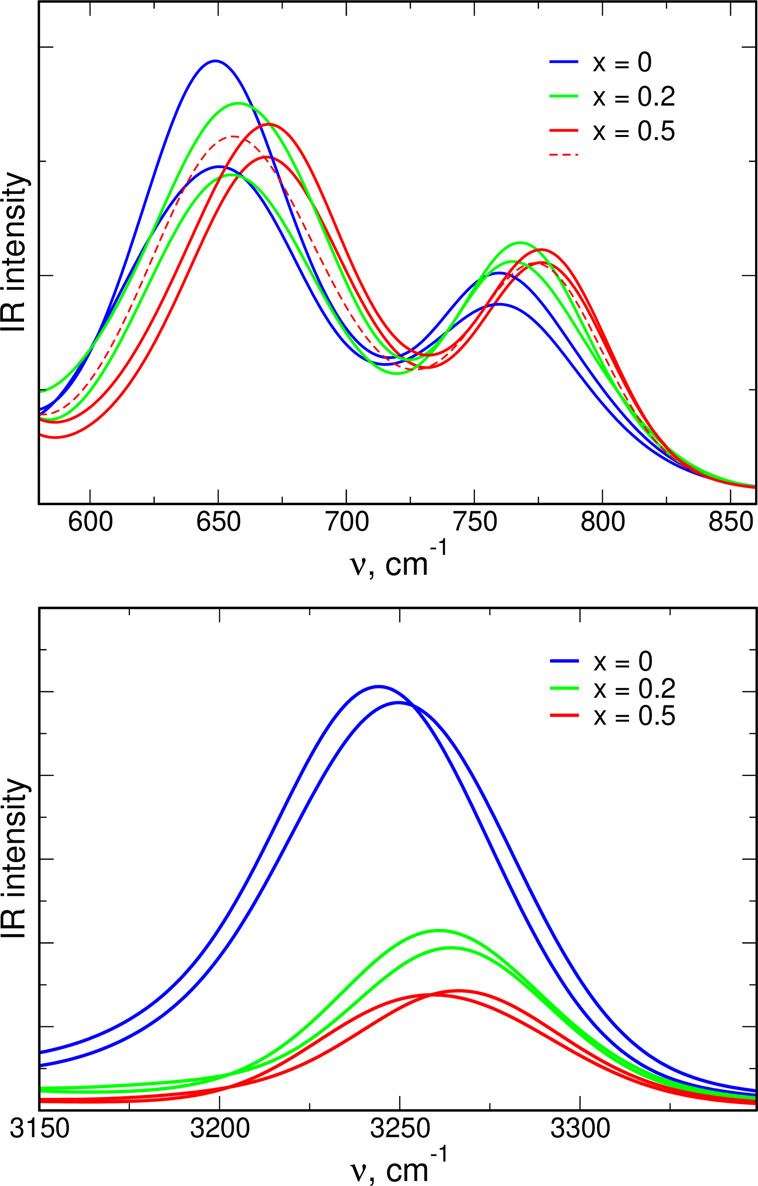
\includegraphics[width=0.4\textwidth]{img/4-ir-spectra-from-aimd-simulations/1-emim-fsi/spectra-aimd.png}
    \caption{IR spectra obtained from AIMD simulations for electrolytes with different mole fractions of NaFSI}
    \label{fig:emim-fsi-spectra-aimd}
\end{figure}

In experimental work~\cite{na-il-1} Raman spectra for the band at 730~cm$^{-1}$ were obtained. However, the ab initio calculation of polarizability needed for obtaining theoretical Raman spectrum would significantly increase the computational effort of the simulation. Fortunately, the band at 730~cm$^{-1}$ for EMIM-FSI is also active in the IR spectrum. Determination of the dipole moment does not affect the computational cost. Therefore, in this work only the IR spectrum is calculated, assuming that the shifts of the band position in IR will be a~good estimate of the effect observed in Raman spectrum.

Spectra from AIMD simulations are systematically redshifted to frequencies lower about 80~cm$^{-1}$ with respect to the experimental spectrum and are presented in Figure~\ref{fig:emim-fsi-spectra-aimd}. The upper panel presents the mentioned region and has been discussed in the Master Thesis, here is will be only noticed that the experimentally observed blue shift of this band with increasing salt concentration was correctly reproduced. Calculated shifts: 7-8~cm$^{-1}$ and 20~cm$^{-1}$ for systems with $x = 0.2$ and $x = 0.5$, respectively, stand in a~good agreement with experimental data from~\cite{na-il-1}: 7~cm$^{-1}$ for $x = 0.2$ and 17~cm$^{-1}$ for $x = 0.5$. One of the systems with $x = 0.5$ (shown in dashed line) is an outlier, with RDFs differing from other electrolytes with this concentration (Figures~\ref{fig:emim-fsi-rdf} and~\ref{fig:emim-fsi-rdf-na-na}) and therefore it was excluded from further analysis.

\begin{figure}[H]
    \centering
    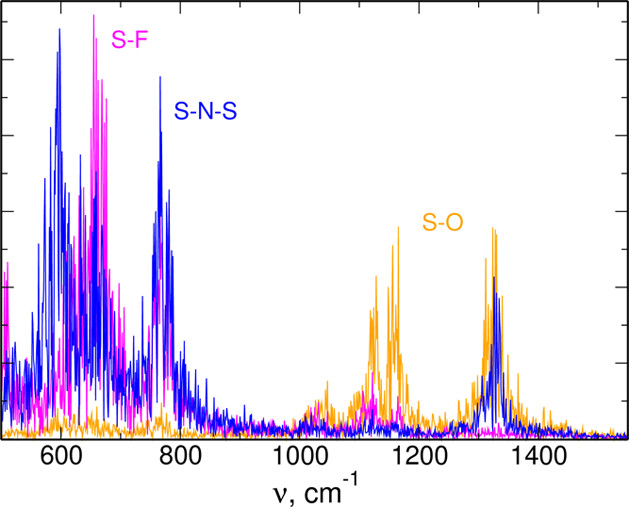
\includegraphics[width=0.4\textwidth]{img/4-ir-spectra-from-aimd-simulations/1-emim-fsi/fourier-samples.png}
    \singlespacing
    \caption{Sample Fourier  transforms of S-O and S-F bond length and S-N-S angle for selected FSI$^{-}$ anion}
    \label{fig:emim-fsi-fourier-samples}
\end{figure}

The bottom panel of Figure~\ref{fig:emim-fsi-spectra-aimd} presents the region of the C-H stretching band in the EMIM$^{+}$ cation. These cations do not interact directly with sodium, however a~blue shift of positions for the maximum is observed. It is probably caused by changes in hydrogen bonding in the system - interactions between FSI$^{-}$ anion with sodium cations are stronger than HBs. Thus with growing concentration of NaFSI less FSI$^{-}$ are available for HBs and the C-H stretches are less involved in HBs. Their frequencies move towards higher values, returning to the values of "free" C-H vibrations. This result is corroborated with changes in the H-O RDF in Figure~\ref{fig:emim-fsi-rdf} with decreasing first maximum with NaFSI concentration increase. The effects of hydrogen bonding on C-H vibrations in EMIM$^{+}$ cation will be addressed in section~\ref{section:il-h2o-ir}.

These results demonstrate that AIMD is able to correctly reproduce shifts observed in vibrational spectra. Oscillations in the system change periodically structural parameters such as bond lengths or angles. Thus, Fourier transforms (FTs) of these magnitudes should be able to catch the frequencies of normal nodes in which these local oscillations contribute. Therefore, to have a~better insight into relation between local interactions and spectral properties, such analysis for NaFSI in EMIM-FSI IL was made. Example FTs for S-O, S-F bond lengths and S-N-S angle are presented in Figure~\ref{fig:emim-fsi-fourier-samples}. From this relations it is seen that the S-F stretching with some contributions of S-N-S angle bending contribute to the band at 650~cm$^{-1}$.

\begin{figure}[ht]
    \centering
    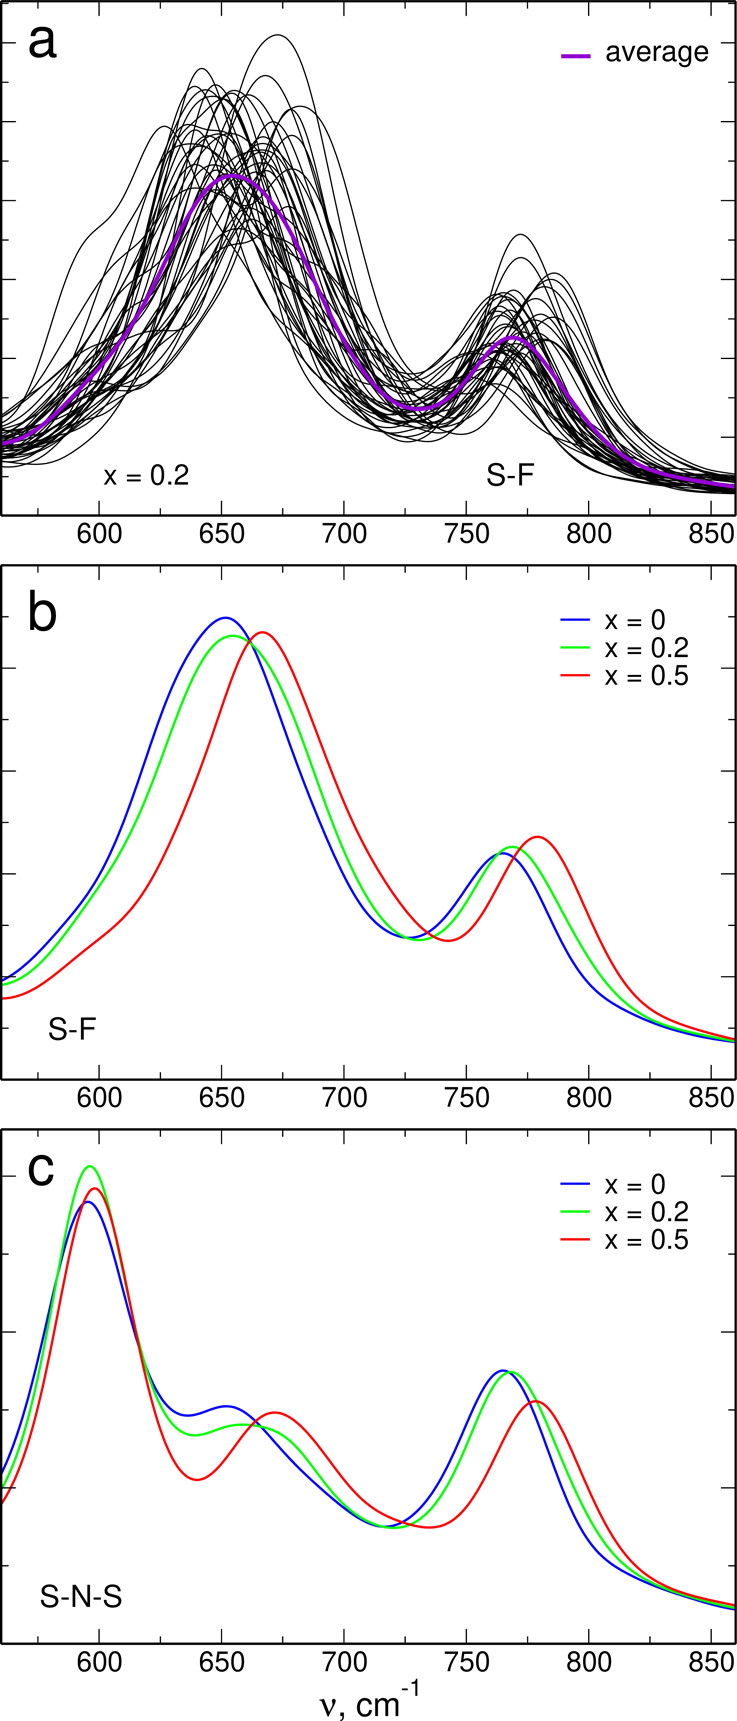
\includegraphics[width=0.4\textwidth]{img/4-ir-spectra-from-aimd-simulations/1-emim-fsi/fourier-individual.png}
    \caption{Fourier transorms of the S-F bond length for all FSI$^{-}$ anions in $x = 0.2$ system (a), average values for Fourier transforms of S-F length (b) and S-N-S angles (c) for different salt concentrations}
    \label{fig:emim-fsi-fourier-individual}
\end{figure}

FTs for all S-F bonds in the $x = 0.2$ system are presented in Figure~\ref{fig:emim-fsi-fourier-individual}a. It is visible that positions of the maxima for individual bonds vary in the broad range of about~70~cm$^{-1}$. The averages for S-F angles are shown in Figure~\ref{fig:emim-fsi-fourier-individual}b. It is clear that these FTs catch the frequencies of normal nodes, as the shifts of the maxima here are analogous to the shifts observed in the IR spectrum.


To check correlations between vibrational frequencies and the local structure, data for several selected FSI$^{-}$ anions are plotted in Figure~\ref{fig:emim-fsi-fourier-rdf}. There are three groups - anions with oscillations close to average frequency (brown lines), these blue-shifted (cyan lines) and red-shifted (orange lines) with respect to the average frequency of S-F stretching. The same colours are used for S-N-S bending in Figure~\ref{fig:emim-fsi-fourier-rdf}b, and here the behaviour is identical, what suggests that the frequencies of S-F and S-N-S oscillations are correlated. For these selected anions in Figure~\ref{fig:emim-fsi-fourier-rdf}c integrated RDFs for O-Na pairs are plotted. This picture shows that there is a~correlation between shift of the individual frequency and the interaction with sodium cation - the anions with frequencies blue shifted with respect to the average value are interacting with more Na$^{+}$ cations while the anions with frequencies red shifted with respect to the average value do not have Na$^{+}$ cations in the first coordinaiton shell.

\begin{figure}
    \centering
    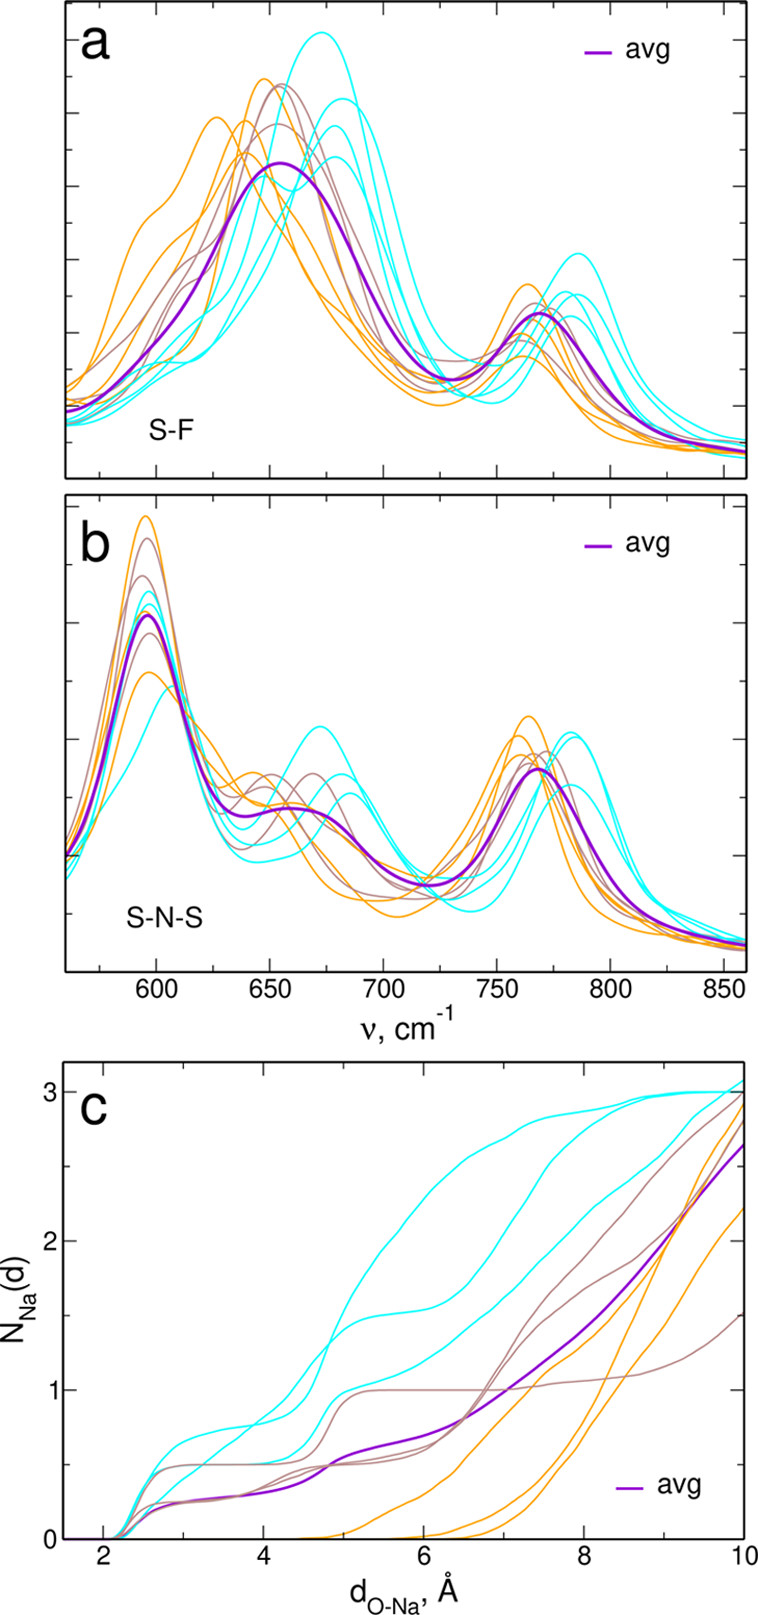
\includegraphics[width=0.4\textwidth]{img/4-ir-spectra-from-aimd-simulations/1-emim-fsi/fourier-rdf.png}
    \caption{Fourier transforms of the (a) S-F bond length and (b) S-N-S angle for selected FSI$^{-}$ anions in the $x = 0.2$ electrolyte and integrated (c) O-Na RDFs for selected anions}
    \label{fig:emim-fsi-fourier-rdf}
\end{figure}

Examples of mentioned anions in different environents are shown in Figure~\ref{fig:emim-fsi-environments}. The top panel presents an anion which has S-F stretching frequency red shifted with respect to average value (not interacting with Na$^{+}$), the middle the one with frequency close to average (weakly interacting with Na$^{+}$) and the bottom the one that has frequency blue shifted with respect to the average value (strongly interacting with Na$^{+}$). Here, weak interaction means that anion interacts with one Na$^{+}$ cation with geometry corresponding to the type III (Figure~\ref{fig:emim-fsi-na-fsi-conformers}) and the strong interaction means interacting simultaneously with two Na$^{+}$ cations (right panel of bottom row of Figure~\ref{fig:emim-fsi-environments}) or with one cation in the stronlgy bound complex of type~I (left panel).

\begin{figure}[ht]
    \centering
    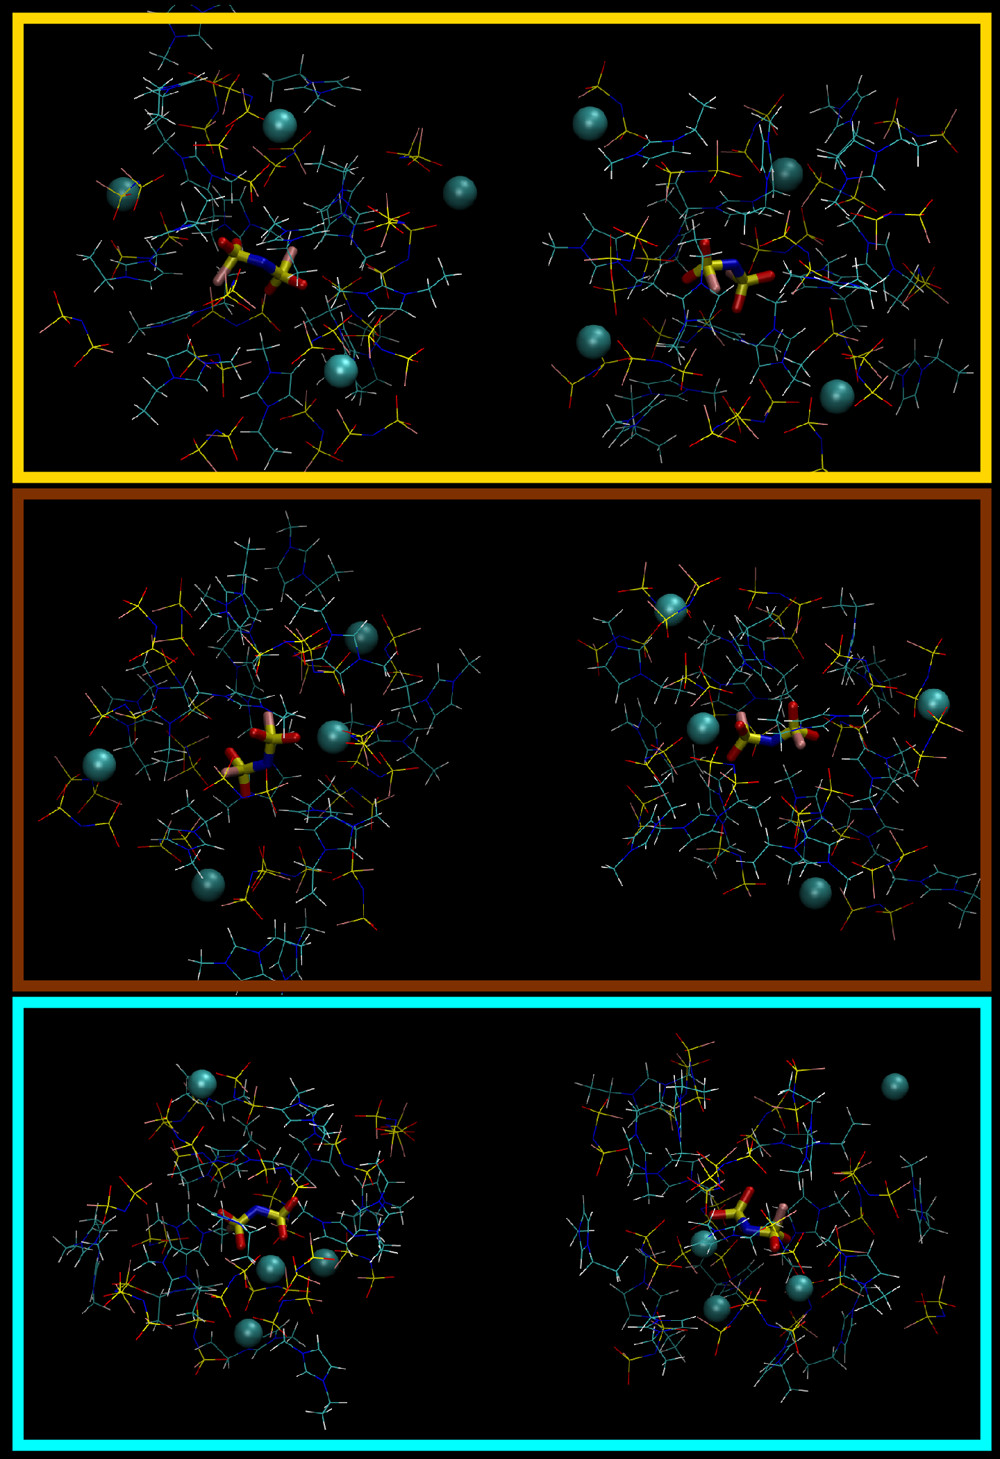
\includegraphics[width=0.4\textwidth]{img/4-ir-spectra-from-aimd-simulations/1-emim-fsi/environments.png}
    \caption{Local environment of selected FSI$^{-}$ anions in the $x = 0.2$ system}
    \label{fig:emim-fsi-environments}
\end{figure}

Thus, here it has been shown that AIMD is able to correctly reproduce effects observed experimentally in IR spectra. What is more, as it has been seen, FTs of geometrical parameters of the system are an additional tool for analysis of vibrational spectra and looking for relations between shifts and chemical environment of molecules. It is confirmed by studying average FTs: for them, the behaviour of maximas positions is analogous to this observed in the IR spectrum.

\cleardoublepage